\chapter{Metodi di decomposizione}

\section{Dantizg-Wolfe Decomposition}
Si consideri il seguente problema di programmazione lineare:
\begin{equation*}
	(P)
	\begin{cases}
		Min\ cx \\
		\ \ \ Ax=b
		\ \ \ x\in X
	\end{cases}
	A\textnormal{ è ($m$ x $n$)}
\end{equation*}
dove $X$ è un insieme \textit{poliedrico convesso limitato} che rappresenta vincoli aventi una "speciale" struttura.

Per il teorema della rappresentazione, essendo per ipotesi $X$ un insieme limitato, detti $x^{1},x^{2},\dots,x^{t}$ i punti estremi di $X$ allora ogni $x\in X$ può essere rappresentato come:
\begin{flalign*}
	& x=\sum_{j=1}^{t}\lambda_{j}x^{j} \\
	& s.t.\ \sum_{j=1}^{t}\lambda_{j}=1 \\
	& \ \ \ \ \ \lambda_{j}\ge 0,\ j=1,\dots,t
\end{flalign*}
Sostituendo $x$ così definito in $P$ si ottiene la seguente formulazione equivalente di $P$ nelle variabili $\lambda_{1},\lambda_{2},\dots,\lambda_{t}$.

\begin{numcases}{P'}
		z'=Min\ \sum_{j=1}^{t}(cx^{j})\lambda_{j} \\
		s.t.\ \sum_{j=1}^{t}(Ax^{j})\lambda_{j}=b \label{eq:5.2} \\
		\ \ \ \ \ \sum_{j=1}^{t}\lambda_{j}=1 \label{eq:5.3} \\
		\ \ \ \ \ \ \ \ \ \ \lambda\ge 0,\ j=1,\dots,t
\end{numcases}

\subsection{Metodo di solzione di $\boldsymbol{P'}$}
$P'$ non può essere risolto direttamente poichè il numero $t$ di punti estremi di $X$ è (di solito) molto grande e tali punti non possono essere enumerati a priori.

Si cerca quindi di risolvere $P'$ senza dover generare tutti i punti estremi di $X$.

\newpage
\subsubsection{Schema dell'algoritmo}
\begin{enumerate}
	\item Problema Master
		\begin{itemize}
			\item Si risolva $P'$ usando un insieme limitato di $k$ punti estremi $x^{1},\dots,x^{k}$ dove $k\ll t$.
			\item Sia $(w,\alpha)$ la soluzione duale ottima di $P'$ usando i $k$ punti estremi generati.\\
			$w=(w_{1},w_{2},\dots,w_{t})$ variabile duale dei vincoli \ref{eq:5.2} e $\alpha$ variabile duale del vincolo \ref{eq:5.3}.
			\begin{equation*}
				D'
				\begin{cases}
					Max\ w b+\alpha \\
					s.t.\ \ w(Ax^{j})+\alpha\le cx{j},\ j=1,\dots,k \\
					\ \ \ \ \ \ w\in\mathscr{R}^{m},\ \alpha\in\mathscr{R} \\
				\end{cases}
			\end{equation*}
		\end{itemize}
	\item Ottimalità della soluzione del Master $P'$\\
	La soluzione ottima di $P'$ è ottima per l'intero problema se e solo se $(w,\alpha)$ soddisfa i vincoli duali dei punti estremi $x^{k+1},x^{k+2},\dots,x^{t}$ non considerati di $P'$, ovvero:
	\begin{equation*}
		w(Ax^{j})+\alpha\le cx^{j},\ j=k+1,\dots,t
	\end{equation*}
	In altri termini, la soluzione di $P'$ è ottima e $(w,\alpha)$ è ottima per $D'$ se
	\begin{equation}
		z_{j}-c_{j}=w(Ax^{j})+\alpha-cx^{j}=(w A-c)x^{j}+\alpha\le 0,\ j=k+1,\dots,t \label{eq:5.5}
	\end{equation}
	Per verificare se le \ref{eq:5.5} sono soddisfatte o violate è sufficiente cercare (se esiste) il punto estremo di $X$ che viola le \ref{eq:5.5}.\\
	Tale punto estremo, se esiste, sarà la soluzione ottima di costo positivo del seguente sottoproblema $SP$:
	\begin{equation*}
		SP
		\begin{cases}
			z_{SP}=Max\ (w A-c)x+\alpha \\
			\ \ \ \ \ \ \ \ \ s.t.\ \ x\in X
		\end{cases}
	\end{equation*}
	sia $x^{*}$ la soluzione ottima di $SP$
	\item Se $z_{SP}>0$ allora la corrente soluzione duale $(w,\alpha)$ viola il vincolo \ref{eq:5.5} per il punto estremo $x^{*}$ di $X$.
	
	Poni $k=k+1$, $x^{k}=x^{*}$ e ritorna allo step 1.\\
	Se $z_{SP}=0$ allora $(w,\alpha)$ soddisfa i vincoli duali \ref{eq:5.5} per i punti estremi non considerati da $P'$, quindi la soluzoine di $P'$ è ottima: \textit{stop}.
\end{enumerate}
Potrebbe risultare computazionalmente proibitivo raggiungere la condizione di ottimalità a causa dell'evelato numero di punti estremi.

\clearpage
\subsection{Lower Bound}
Ad ogni interazione è possibile calcolare un lower bound $LB$ al costo ottimo $z^{*}$ di $P$ e quindi si può terminare l'algoritmo quando il costo di $z'$ di $P'$ limitato a $k$ punti estremi è sufficientemente "vicino" a $LB$; ad esempio, quando
\begin{equation}
	\frac{z'-LB}{LB}\le TOL \label{eq:5.6}
\end{equation}
dove $TOL$ è definito a-priori dall'utente.
\subsubsection{Calcolo del lower bound $\boldsymbol{LB}$}
Si noti che per come è definito $SP$ si ha che
\begin{equation*}
	(w A-c)x+\alpha\le z_{SP},\ \forall x\in X
\end{equation*}
o anche
\begin{equation}
	w Ax-cx+\alpha\le z_{SP}, \ \forall x\in X \label{eq:5.7}
\end{equation}
Si consideri una qualunque soluzione $x$ di $P$ (ovvero $x\in X$ e $Ax=b$), dalla \ref{eq:5.7} si ha:
\begin{equation*}
	w b-cx+\alpha\le z_{SP}
\end{equation*}
o anche
\begin{equation*}
	cx\ge\overbrace{w b+\alpha}^{z'}-z_{SP}=z'-z_{SP}
\end{equation*}
Qunidi $LB=w b+\alpha-z_{SP}$ è un lower bound valido e l'algoritmo può terminare qualora la soluzione $z'$ del problema master verifichi la \ref{eq:5.6}.

\subsection{Esempio}
\begin{flalign*}
		& Min\ -2x_{1}-x_{2}-x_{3}+x_{4} \\
		& s.t. \ \ \begin{rcases}
					x_{1}+x_{3}\le 2 \\
					x_{1}+x_{2}+2x_{4}\le 3  \\
			   \end{rcases} Ax\le b \\
		& \ \ \ \ \ \ \ \begin{rcases}
				   x_{1}\le 2 \\
				   x_{1}+2x_{2}\le 5 \\
				   -x_{3}+x_{4}\le 2 \\
				   2x_{3}+x_{4}\le 6 \\
				   x_{1},x_{2},x_{3},x_{4}\ge 0
			   \end{rcases}x\in X
\end{flalign*}
Quindi, formalmente, $P$ può essere scritto come
\begin{equation*}
	P
	\begin{cases}
		Min\ cx \\
		\ \ \ \ \ \ \ Ax+s=b \\
		\ \ \ \ \ \ \ x\in X, s\ge 0 \ x\ge 0
	\end{cases}
\end{equation*}
Ogni $(x_{1},x_{2},x_{3},x_{4})\in X$ ha le prime due componenti in $X_{1}$ e le ultime due in $X_{2}$ come mostrato in seguito.\\
\centerline{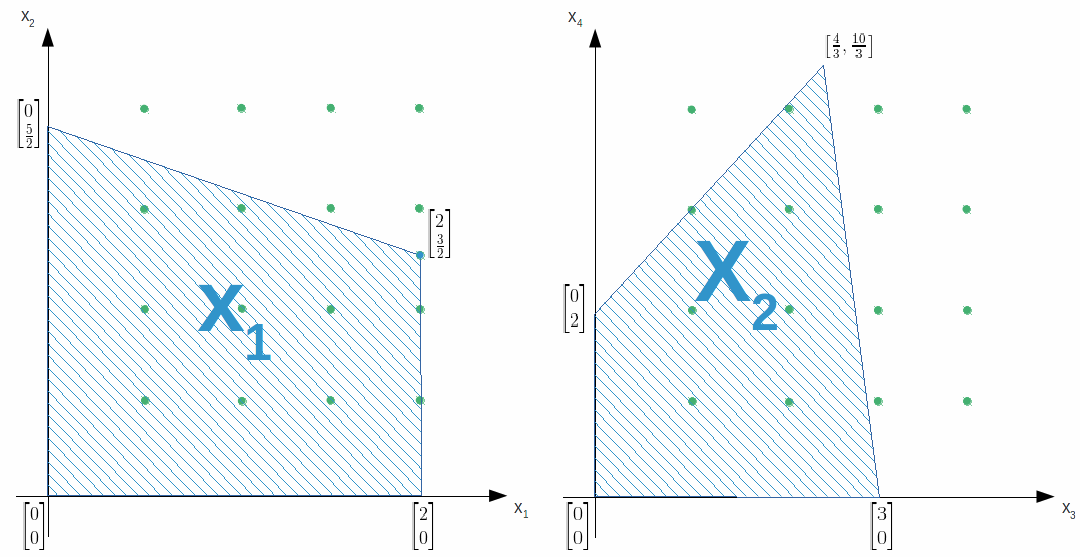
\includegraphics[height=7cm]{images/graph51.png}\label{fig:5.1.3}}\\
\begin{flalign*}
	& X_{1}=\{(x_{1},x_{2}):x_{1}\le 2, x_{1}+2x_{2}\le 5; \ x_{1},x_{2}\ge 0\} \\
	& X_{2}=\{(x_{3},x_{4}):-x_{3}+x_{4}\le 2,\ 2x_{3}+x_{4}\le 6,\ x_{3},x_{4}\ge 0\}
\end{flalign*}
\subsection{Inizializzazione}
Siano $x^{1},x_{2},\dots,x_{t}$ i punti estremi di $X$.\\
Poniamo $\hat{c}_{j}=cx_{j}$ il costo del punto estremo $x^{j}$, $j=1\,dots,t$
\begin{equation*}
	P'
	\begin{cases}
		Min\ \sum_{j=1}^{t}\hat{c}_{j}\lambda_{j} \\
		\ \ \ \ \ \ \ \sum_{j=1}^{t}(Ax^{j})\lambda_{j}+s=b \\
		\ \ \ \ \ \ \ \sum_{j=1}^{t}\lambda_{j}=1 \\
		\ \ \ \ \ \ \ \ \ \ \ \ \lambda_{j}\ge 0,\ j=1,\dots,t
	\end{cases}
\end{equation*}
Si può partire con il punto estremo $x^{1}=(0,0,0,0)$ di costo $\hat{c}_{1}=0$
\begin{equation*}
	P'
	\begin{cases}
		z^{1}=Min\ 0\lambda_{1} \\
		s_{1}=2\ \ \ \ \ \ \ \ \ \ \ \ w_{1}\\
		s_{3}=3\ \ \ \ \ \ \ \ \ \ \ \ w_{2}\\
		\lambda_{1}=1\ \ \ \ \ \ \ \ \ \ \ \ \alpha\\
		s_{1},s_{2},\lambda_{1}\ge 0
	\end{cases}
\end{equation*}
Ottimo: $\lambda_{1}=1$, $s_{1}=2$, $s_{2}=3$, $z^{1}=0$ e $(w_{1},w_{2},\alpha)=(0,0,0,0)$.\\

La soluzione primale di $P$ di costo $z^{1}=0$ è $x=\lambda_{1}x^{1}=0x^{1}=(0,0,0,0)$.

\subsubsection{Iterazione 1}
\begin{flalign*}
	& SP\ \ \ \ \ \ \ \ \ Max\ (w A-c)x+\alpha \\
	& \ \ \ \ \ \ \ \ \ \ \ \ \ \ \ \ \ \ \ \ \ s.t.\ \ x\in X 
\end{flalign*}
Poichè $(w_{1},w_{2},\alpha)=0$
\begin{flalign*}
& SP\ \ \ \ \ \ \ \ \ Max\ 2x_{1}+x_{2}+x_{3}-x_{4}+0 \\
& \ \ \ \ \ \ \ \ \ \ \ \ \ \ \ \ \ \ \ \ \ x\in X \textnormal{ o }(x_{1},x_{2})\in X_{1},\ (x_{3},x_{4})\in X_{2}
\end{flalign*}
$SP$ è separabile nei vettori $(x_{1},x_{2})\in X_{1}$ e $(x_{3},x_{4})\in X_{2}$ per cui, come si vede in \ref{fig:5.1.3}, si ha che una soluzione ottima di $SP$ è data dal punto estremo
\begin{equation*}
	x^{2}=(2,\frac{3}{2},3,0)
\end{equation*}
$z_{2}-\hat{c}_{2}=(w A-c)x^{2}+\alpha=-cx^{2}=\frac{17}{2}>0$\\
Lower bound $z^{1}-(z_{2}-\hat{c}_{2})=-\frac{17}{2}=-8.5$ e $x_{2}$ entra nel Master

\clearpage
\subsubsection{Nuovo Master}
\begin{equation*}
	P'
	\begin{cases}
		Min\ \ \hat{c}_{1}\lambda_{1}+\hat{c}_{2}\lambda_{2}\\
		\ \ \ \ \ \ \ (Ax^{1})\lambda_{1}+(Ax_{2})\lambda_{2}+s=b \\
		\ \ \ \ \ \ \ \ \ \ \ \ \ \ \ \lambda_{1}+\lambda_{2}=1 \\
		\ \ \ \ \ \ \ \ \ \ \ \ \ \ \ \lambda_{1}+\lambda_{2}\ge 0,\ s\ge 0
	\end{cases}
\end{equation*}
Nel calcolo in esame $Ax^{1}=\begin{bmatrix}0\\0\end{bmatrix}$, $Ax_{2}=\begin{bmatrix}5\\\frac{7}{2}\end{bmatrix}$, quindi
\begin{equation*}
	P'
	\begin{cases}
		z^{1}=Min\ 0\cdot\lambda_{1}+(-\frac{17}{2})\lambda_{2} \\
		\ \ \ \ \ \ \ \ \ \ \ \ \ \ 0\cdot\lambda_{1}+5\lambda_{2}+s_{1}=2 \\
		\ \ \ \ \ \ \ \ \ \ \ \ \ \ 0\cdot\lambda_{1}+\frac{7}{2}\lambda_{2}+s_{2}=3 \\
		\ \ \ \ \ \ \ \ \ \ \ \ \ \ \lambda_{1}+\lambda_{2}=1 \\
		\ \ \ \ \ \ \ \ \ \ \ \ \ \ \lambda_{1},\lambda_{2},s_{1},s_{2}\ge 0
	\end{cases}
\end{equation*}
Ottimo: $\lambda_{1}=\frac{3}{5}$, $\lambda_{2}=\frac{2}{5}$, $s_{1}=0$, $s_{2}=\frac{2}{5}$, $z^{1}=-\frac{17}{5}$.
\begin{equation*}
	(w_{1},w_{2},\alpha)=(-\frac{17}{10},0,0)
\end{equation*}
La soluzione primale di $P$ di costo $z^{1}=-\frac{17}{6}=-3\cdot 4$ è
\begin{equation*}
	x=\lambda_{1}x^{1}+\lambda_{2}x^{2}=\frac{5}{3}+\frac{2}{5}x^{2}=(\frac{4}{5},\frac{3}{5},\frac{6}{5},0)
\end{equation*}

\subsubsection{Iterazione 2}
\begin{equation*}
	SP
	\begin{cases}
		Max\ \ (w A-c)x+\alpha \\
		\ \ \ \ \ \ \ \ \ s.t. \ x\in X
	\end{cases}
\end{equation*}
$(w A-c)=(\frac{3}{10},1,-\frac{7}{10},-1)$
\begin{equation*}
	SP
	\begin{cases}
		Max\ \frac{3}{10}x_{1}+x_{2}-\frac{7}{10}x_{3}-x_{4}+0 \\
		\ \ \ \ \ \ \ \ s.t.\ (x_{1},x_{2})\in X_{1},\ (x_{3},x_{4})\in X_{2}
	\end{cases}
\end{equation*}
Ottimo $x^{3}=(0,\frac{5}{2},0,0)$ e $z-\hat{c}_{3}=\frac{5}{2}>0$.\\
Lower bound $z^{1}-(z_{3}-\hat{c}_{3})=-\frac{17}{5}-\frac{5}{2}=-5.4$

\subsubsection{Nuovo Master}
\begin{equation*}
	P'
	\begin{cases}
		Min\ \hat{c}_{1}\lambda_{1}+\hat{c}_{2}\lambda_{2}+\hat{c}_{3}\lambda_{3}\\
		\ \ \ \ \ \ \ (Ax^{1})\lambda_{1}+(Ax^{2})\lambda_{2}+(Ax^{3})\lambda_{3}+s=b \\
		\ \ \ \ \ \ \ \lambda_{1}+\lambda_{2}+\lambda_{3}=1 \\
		\ \ \ \ \ \ \ \lambda_{1},\lambda_{2},\lambda_{3},s\ge 0
	\end{cases}
\end{equation*}
$\hat{c}_{3}=cx^{3}=-\frac{5}{2}$, $Ax^{3}=\begin{Bmatrix}0\\\frac{5}{2}\end{Bmatrix}$, quindi
\begin{equation*}
	P'
	\begin{cases}
		z^{1}=Min\ 0\cdot\lambda_{1}-\frac{17}{2}\lambda_{2}-\frac{5}{2}\lambda_{3} \\
		\ \ \ \ \ \ \ \ \ \ \ \ \ \  0\cdot\lambda_{1}+5\lambda_{2}+0\cdot\lambda_{3}+s_{1}=2 \\
		\ \ \ \ \ \ \ \ \ \ \ \ \ \  0\cdot\lambda_{1}+\frac{7}{2}\lambda_{2}+\frac{5}{2}\lambda_{3}+s_{2}=3 \\
		\ \ \ \ \ \ \ \ \ \ \ \ \ \ \lambda_{1}+\lambda_{2}+\lambda_{3}=1
	\end{cases}
\end{equation*}
Ottimo: $\lambda_{1}=0$, $\lambda_{2}=\frac{2}{5}$, $\lambda_{3}=\frac{3}{5}$, $s_{1}=0$, $s_{1}=\frac{1}{10}$ e $z^{1}=-4.9$, inoltre, $(w_{1},w_{2},\alpha)=(-\frac{6}{5},0,-\frac{5}{2})$.\\
Lo soluzione di $P$ di costo $-4.9$ è $x=\lambda_{2}x^{2}+\lambda_{3}x^{3}=(\frac{4}{5},21,\frac{6}{5},0)$

\subsubsection{Iterazione 3}
\begin{equation*}
	SP
	\begin{cases}
		Max\ (w A-c)x+\alpha \\
		\ \ \ \ \ \ \ \ s.t.\ x\in X
	\end{cases}
\end{equation*}
$(w A-c)=(\frac{4}{5},1,-\frac{1}{5},-1)$
\begin{equation*}
	SP
	\begin{cases}
		z_{SP}=Max\ \frac{4}{5}x_{1}+x_{2}-\frac{1}{5}x_{3}-x{4}-\frac{5}{2} \\
		\ \ \ \ \ \ \ \ (x_{1},x_{2})\in X_{1},\ (x_{3},x_{4})\in X_{2}
	\end{cases}
\end{equation*}
$x^{4}=(2,\frac{3}{2},0,0)$ e $z_{SP}=(z_{4}-\hat{c}_{4})=\frac{3}{5}$.\\
Lower Bound $z^{1}-(z_{4}-\hat{c}_{4})=-4.9-\frac{3}{5}=-5.5$

\subsubsection{Nuovo Master}
\begin{flalign*}
	& Ax^{4}=\begin{Bmatrix}2\\\frac{7}{2}\end{Bmatrix} \\
	& cx^{4}=-\frac{11}{2}
\end{flalign*}
\begin{equation*}
	P
	\begin{cases}
		z^{1}=Min\ 0\cdot\lambda_{1}-\frac{17}{2}\lambda_{2}-\frac{5}{2}\lambda_{3}-\frac{11}{2}\lambda_{4} \\
		\ \ \ \ \ \ \ \ \ \ \ \ \ \ 0\cdot\lambda_{1}+5\lambda_{2}+0\cdot\lambda_{3}+2\lambda_{4}+s_{1}=2 \\
		\ \ \ \ \ \ \ \ \ \ \ \ \ \ 0\cdot\lambda_{1}+\frac{7}{2}\lambda_{2}+\frac{6}{2}\lambda_{3}+\frac{7}{2}\lambda_{4}+s_{2}=3 \\
		\ \ \ \ \ \ \ \ \ \ \ \ \ \ \lambda_{1}+\lambda_{2}+\lambda_{3}+\lambda_{4}=1 \\
		\ \ \ \ \ \ \ \ \ \ \ \ \ \ \lambda_{1},\dots,\lambda_{4},s_{1},s_{2}\ge 0
	\end{cases}
\end{equation*}
Ottimo $\lambda_{1}=0$, $\lambda_{2}=\frac{1}{3}$, $\lambda_{3}=\frac{1}{6}$, $\lambda_{4}=\frac{1}{2}$, $z^{1}=-5$.

$(w_{1},w_{2},\alpha)=(-1,-1,0)$

La soluzione di $P$ di costo $-$ è $x=\lambda_{2}x^{2}+\lambda_{3}x^{3}+\lambda_{4}x^{4}=\frac{1}{3}x^{2}+\frac{1}{6}x_{3}+\frac{1}{2}x^{4}=(1,2,1,0)$

\subsubsection{Iterazione 4}
\begin{equation*}
	SP
	\begin{cases}
		Max\ (w A-c)x+\alpha \\
		\ \ \ \ \ \ \ x\in X
	\end{cases}
\end{equation*}
$(w A-c)=(0,0,0,-3)$
\begin{equation*}
	SP
	\begin{cases}
		z_{SP}=Max\ 0\cdot x_{1}+0\cdot x_{2}+0\cdot x_{3}-3x_{4}+0 \\
		\ \ \ \ \ \ \ \ (x_{1},x_{2})\in X_{1},\ (x_{3},x_{4})\in X_{2} 
	\end{cases}
\end{equation*}
Ottimo $z_{SP}=0$: \textit{stop}.

Lower Bound $z^{1}-z_{SP}=z^{1}=-s$.

Quindi la soluzione ottima del problema originario è
\begin{equation*}
	x=\frac{1}{3}x^{2}+\frac{1}{6}x^{3}+\frac{1}{2}x^{4}=(1,2,1,0)
\end{equation*}
\centerline{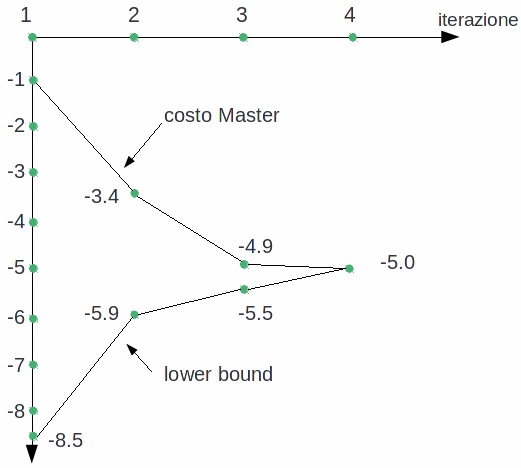
\includegraphics[height=7cm]{images/graph52.png}}

\section{Struttura Diagonale a blocchi di X}
È il caso in cui $X$ può essere decomposto in $T$ sottoinsiemi $X_{1},X_{2},\dots,X_{T}$ e il vettore delle varibili in $T$ vettori $x_{1},x_{2},\dots,x_{T}$ tali che $x_{k}\in X_{k}$, $k=1,\dots,T$.\\
Indichiamo con $c_{k}$ il vettore dei costi e con $A_{k}$ la sottomatrice di $A$ relativa alle variabili $x_{k}$, $k=1,\dots,T$.\\
Il problema $P$ si può scrivere come seuge:
\begin{equation*}
	P
	\begin{cases}
	Min\ c_{1}x_{1}+c_{2}x_{2}+\dots+c_{T}x_{T}=Min\ \sum_{k=1}^{T}c_{k}X_{k} \\
	\ \ \ \ \ \ \ A_{1}x_{1}+A_{2}x_{2}+\dots+a_{T}x_{T}=b\ \sum_{k}A_{k}x_{k}=b \\
	\ \ \ \ \ \ \ B_{1}x_{1}\ \ \ \ \ \ \ \ \ \ \ \ \ \ \ \ \ \ \ \ \ \ \ \ \ \ \ \ =b_{1} \\
	\ \ \ \ \ \ \ \ \ \ \ \ \ \ \ \ \ B_{2}x_{2}\ \ \ \ \ \ \ \ \ \ \ \ \ \ \ \ \ \ =b_{2} \\
	\ \ \ \ \ \ \ \ \ \ \ \ \ \ \ \ \ \ \ \ \ \ \ \ \ \ \ \ddots\ \ \ \ \ \ \ \ \ \ \ \ \ \vdots \\
	\ \ \ \ \ \ \ \ \ \ \ \ \ \ \ \ \ \ \ \ \ \ \ \ \ \ \ \ \ \ \ \ \ \ B_{T}x_{T}=b_{T}\\
	\ \ \ \ \ \ \ x_{1},x_{2},\dots,x_{T}\ge 0
	\end{cases}
\end{equation*}
dove $X_{i}=\{x_{i}:B_{i}x_{i}=b_{i},\ x_{i}\ge 0\}$, $i=1,\dots,T$.\\
L'algoritmo descritto in precedenza può essere ulteriormente specializzato per sfruttare la particolare struttura che definisce $x\in X$.

Supponiamo che ogni insieme $X_{i}$ sia limitato.\\
Per ogni sottoinsieme $X_{k}$ (limitato) indichiamo con $x^{1}_{k},x^{2}_{k},\dots,x^{t_{k}}_{k}$ i punti estremi, quindi $x_{k}\in X_{k}$ può essere rappresentato come
\begin{equation*}
	\begin{rcases}
		x_{k}=\sum_{j=1}^{t_{k}}\lambda_{kj}x_{k}^{j}\ \ \ \ \ \ \ \ \ \ \ \ \ \ \ \ \ \ \ \ \ \\
		\sum_{j=1}^{t_{k}}\lambda_{kj}=1\ \ \ \ \ \ \ \ \ \ \ \ \ \ \ \ \ \ \\
		\lambda_{kj}\ge 0,\ j=1,\dots,t_{k}
	\end{rcases}
	k=1,\dots,T
\end{equation*}
Sostituendo ogni $x_{k}$ con $k=1,\dots,T$ così definito in $P$ si ha
\begin{numcases}{P'}
	z'=Min\ \sum_{k=1}^{T}(\sum_{j=1}^{t_{k}}(c_{k}x_{k}^{j})\lambda_{kj}) \\
	\ \ \ \ \ \ \ \ \ \ \ \ \ \ \sum_{k=1}^{T}(\sum_{j=1}^{t_{k}}(A_{k}x_{k}^{j})\lambda_{kj})=b \label{eq:5.9}\\
	\ \ \ \ \ \ \ \ \ \ \ \ \ \ \sum_{j=1}^{t_{k}}\lambda_{kj}=1,\ k=1,\dots,T \label{eq:5.10}\\
	\ \ \ \ \ \ \ \ \ \ \ \ \ \ \lambda_{kj}\ge 0,\ j=1,\dots,t_{k},\ k=1,\dots,T
\end{numcases}
Siano $w=(w_{1},\dots,w_{m})$ e $\alpha=(\alpha_{1},\dots,\alpha_{T})$ le variabili duali, rispettivamente dei vincoli \ref{eq:5.9} e \ref{eq:5.10}.
\begin{equation*}
	D'
	\begin{cases}
		Max\ w b+\sum_{k=1}^{T}\alpha_{k} \\
		\ \ \ \ \ \ \ \ w(A_{k}x_{k}^{j})+\alpha_{k}\le c_{k}x_{k}^{j},\ j=1,\dots,t_{k},\ k=1,\dots,T \\
		\ \ \ \ \ \ \ \ w\in\mathscr{R}^{m},\ \alpha\in\mathscr{R}^{T}
	\end{cases}
\end{equation*}

\subsection{Metodo di soluzione}
Si fa uso della particolare struttura di $X$.
\begin{enumerate}
	\item \textbf{Master problem}\\
	Si risolva $P'$ usando un numero limitato $r_{k}\ll t_{k}$ dei punti estremi di ciascun insieme $X_{k}$, $k=1,\dots,T$.\\
	Sia $(w,\alpha)$ la soluzione del duale del suddetto master.
	\item \textbf{Ottimalità della soluzione del Master}\\
	La soluzione del Master è ottima se $(w,\alpha)$ soddisfa i vincoli duali per i punti estremi non generati; ovvero, se per ogni $k=1,\dots,T$
	\begin{equation*}
		w(A_{k}x_{k}^{j})+\alpha_{k}\le c_{k}x_{k}^{j},\ j=r_{k}\mp 1,\dots,t_{k}
	\end{equation*}
	ovvero se
	\begin{equation*}
			(w A_{k}-c_{k})x_{k}^{j}+\alpha_{k}\le 0,\ j=r_{k}+1,\dots,t_{k}
	\end{equation*}
	Si risolva quindi per ogni $k=1,\dots,T$
	\begin{equation*}
		SP_{k}
		\begin{cases}
			z_{SP}=Max\ (w A_{k}-c_{k})x_{k}+\alpha_{k} \\
			\ \ \ \ \ \ \ \ \ \ \ s.t.\ B_{k}x_{k}=b_{k} \\
			\ \ \ \ \ \ \ \ \ \ \ \ \ \ \ \ \ x_{k}\ge 0
		\end{cases}
	\end{equation*}
	Sia $x_{k}^{*}$ la soluzione ottima.
	\item Se $z_{SP}^{k}\ge 0$, $\forall k:\ stop$ la soluzione è ottima; altrimenti per ogni $k$ per cui $z_{SP}^{k}>0$ poni $r_{k}=r_{k}+1$, $x_{k}^{r_{k}}=x_{k}$ e quindi ritorna al punto 1.
\end{enumerate}

\clearpage
\subsection{Lower Bound}
Come descritto in precedenza, si può terminare l'algoritmo quando il costo $z'$ del Master non dista "troppo" dall'ottimo ovvero quando
\begin{equation*}
	\frac{z'-LB}{LB}\le TOL
\end{equation*}
dove $LB$ può essere così calcolato.
Per come è definito ogni $SP_{k}$, $k=1,\dots,T$, si ha che
\begin{equation*}
	(w A_{k}-c_{k})x_{k}+\alpha_{k}\le z_{SP}^{k},\ k=1,\dots,T
\end{equation*}
o anche
\begin{equation*}
	c_{k}x_{k}\ge w A_{k}x_{k}+\alpha_{k}-z_{SP}^{k},\ k=1,\dots,T
\end{equation*}
sommando
\begin{equation*}
	\sum_{k=1}^{T}c_{k}x_{k}\ge w\sum_{k=1}^{T}A_{k}x_{k}+\sum_{k=1}^{T}A_{k}x_{k}+\sum_{k=1}^{T}\alpha_{k}-\sum_{k=1}^{T}z_{SP}^{k}
\end{equation*}

Si consideri un qualunque $x=(x_{1},...,x_{T})$ che soddisfi $x_{k}\in X_{k}$, $\forall k$ e $A_{1}x_{1}+A_{2}x_{2}+\dots,A_{T}x_{T}=b$ si ha
\begin{equation*}
	\sum_{k=1}^{T}c_{k}x_{k}\ge w b+\sum_{k=1}^{T}\alpha_{k}-\sum_{k=1}^{T}z_{SP}^{k}
\end{equation*}
Quindi $LB=\underbrace{w b+\sum_{k}\alpha_{k}}_{z'}-\sum_{k}z^{k}_{SP}$.\\
$LB$ è un limite inferiore al costo della soluzione ottima.

\section{Assegnamento Generalizzato}
\begin{itemize}
	\item[m] contenitori di capacità $Q_{1},\dots,Q_{m}$
	\item[n] oggetti che devono essere caricati nei contenitori
	\item[$c_{oj}$] costo per caricare l'oggetto $i$ nel contenitore $j$
	\item[$q_{ji}$] spazio del contenitore $j$ occupato da $i$ se $i$ viene caricato nel contenitore $j$.
\end{itemize}
Si vogliono caricare tutti gli oggetti nei contenitori minimizzando il costo complessivo.
\begin{numcases}{P}
	Min\ \sum_{i=1}^{n}\sum_{j=1}^{m}c_{ij}x_{ij} \label{eq:5.12}\\
	\ \ s.t.\ \sum_{j=1}^{m}x_{ij}=1,\ i=1,\dots,n \label{eq:5.13} \\
	\ \ \ \ \ \ \ \ \sum_{i=1}^{n}q_{ij}x_{ij}\le Q,\ j=1,\dots,m \label{eq:5.14}\\
	\ \ \ \ \ \ \ \ \ \ \ \ \ x_{ij}\in\{0,1\},\ \forall i,j \label{eq:5.15}
\end{numcases}
$x_{ij}=1$ se $i$ è caricato nel contenitore $j$; $x_{ij}=0$ altrimenti.

\subsection{Decomposizione Dantzig-Wolfe del GAP}
Indichiamo con $X_{j}$ l'insieme delle soluzioni intere del vincolo \ref{eq:5.14} per il contenitore $j$, $j=1,\dots,m$
\begin{equation*}
	X_{j}=\{x_{j}:\sum_{i=1}^{n}q_{ij}x_{ij}\le Q,\ x_{ij}\in\{0,1\},\ i=1,\dots,n\}
\end{equation*}
dove $x_{j}=(x_{1j},x_{2j},\dots,x_{nj})^{T}$.\\
Siano $x_{j}^{1},x_{j}^{2},\dots,x_{j}^{t_{j}}$ i punti estremi di $conv(X_{j})$.

Per il teorema della rappresentazione abbiamo:
\begin{flalign}
	& \begin{rcases} \label{eq:5.16}
		x_{ij}=\sum_{r=1}^{t_{j}}\lambda_{jr}x_{ij}^{r},\ i=1,\dots,m \\
		\sum_{r=1}^{t_{j}}\lambda_{jr}=1\ \ \ \ \ \ \ \ \ \ \ \ \ \ \ \ \\
		\lambda_{jr}\ge 0\ \ \ \ \ \ \ \ \ \ \ \ \ \ \ \ 
	  \end{rcases} j=1,\dots,m
\end{flalign}
Sostituendo in $P$, definito da \ref{eq:5.12} - \ref{eq:5.15}, $x_{ij}$ secondo \ref{eq:5.16}:
\begin{numcases}{P'}
	Min\ \sum_{i=1}^{n}\sum_{j=1}^{m}c_{ij}\sum_{r=1}^{t_{j}}\lambda_{jr}x_{ij}^{r} \\
	\ \ s.t.\ \sum_{j=1}^{m}\sum_{r=1}^{t_{j}}\lambda_{jr}x_{ij}^{r}=1,\ i=1,\dots,n \\
	\ \ \ \ \ \ \ \ \sum_{r=1}^{t_{j}}\lambda_{jr}=1,\ j=1,\dots,m \\
	\ \ \ \ \ \ \ \ \ \ \ \ \ \lambda_{jr}\in\{0,1\},\ j=1,\dots,m,\ r=1,\dots,t_{j} \label{eq:5.20}
\end{numcases}
I vincoli \ref{eq:5.20} derivano dal fatto che $x_{ij}\in\{0,1\}$.\\

Perché $\lambda_{ji}\in\{0,1\}$ invece di $\lambda_{jr}\ge 0$?

Il motivo è che le soluzioni frazionarie di $\lambda_{jr}$ per un dato $j$ inducono nei \ref{eq:5.20} soluzioni frazionarie di $x_{ij}$.\\
Si consideri il sequente esempio dei \ref{eq:5.20} per un dato $j$ per il quale vengono mostrati $t_{j}=5$ punti estremi di $conv(X_{j})$.
\begin{table}[!h]
	\centering
	\begin{tabular}{c|cccccc}
		& $\lambda_{j1}$ & $\lambda_{j2}$ & $\lambda_{j3}$ & $\lambda_{j4}$ & $\lambda_{j5}$ \\ \cline{1-6}
		$x_{1j}$ & 1 & 1 & 0 & 0 & 1 & \\
		$x_{2j}$ & 0 & 1 & 1 & 0 & 1 & \\
		$\cdot$  & 1 & 0 & 1 & 1 & 0 & \\
		$\cdot$  & 0 & 1 & 0 & 1 & 0 & \\
		$\cdot$  & 1 & 0 & 0 & 1 & 0 & \\
		$x_{6j}$ & 0 & 0 & 1 & 0 & 1 & \\
		& 1 & 1 & 1 & 1 & 1 & = 1
	\end{tabular}
\end{table}
\begin{equation*}
	\lambda_{j1},\dots,\lambda_{j5}\ge 0
\end{equation*}
Ogni soluzione frazionaria di $\lambda$ induce una soluzione frazionaria in $x_{ij}$.

\clearpage
\textbf{Esempio.}

$\lambda_{ji}=\frac{1}{2}$, $\lambda_{j2}=\frac{1}{2}$ e $\lambda_{j3}=\lambda_{j4}=\lambda_{j5}=0$ \\
induce\\
$x_{1j}=1$, $x_{2j}=\frac{1}{2}$, $x_{3j}=\frac{1}{2}$, $x_{4j}=\frac{1}{2}$ e $x_{5j}=0$.\\

Affinchè soluzioni frazionarie $\lambda$ inducano soluzioni intere $x$ è necessario che i punti estremi $x_{j}^{r}$, corrispondenti a $\lambda_{jr}>0$, coincidano; ma ciò non avviene perchè i punti estremi di $conv(X)$ sono ovviamente distinti.

Quindi l'unica possibilità affinchè $x_{ij}\in\{0,1\}$ è che anche $\lambda_{jr}\in\{0,1\}$.\\

$P'$ può essere riscritto come segue:
\begin{numcases}{P'}
	Min\ \sum_{j=1}^{m}\sum_{r=1}^{t_{j}}c(x_{j}^{r})\lambda_{jr} \\
	\ s.t.\  \sum_{j=1}^{m}\sum_{r=1}^{t_{j}}x_{ij}^{r}\lambda_{jr}=1,\ i=1,\dots,n \label{eq:5.22} \\
	\ \ \ \ \ \ \ \ \sum_{r=1}^{t_{j}}\lambda_{jr}=1,\ j=1,\dots,m \label{eq:5.23} \\
	\ \ \ \ \ \ \ \ \ \ \ \ \ \lambda_{jr}\in\{0,1\} \label{eq:5.24}
\end{numcases}
dove $c(x_{j}^{r})=\sum_{i=1}^{n}c_{ij}x_{ij}^{r}$ è il costo del punto estremo $x_{j}^{r}$.\\
Indichiamo con $LP'$ il rilassamento lineare di $P'$ (sostituiamo \ref{eq:5.24} con $\lambda_{jr}\ge 0$).\\
$LP'$ può essere risolto usando il metodo Dantzig-Wolfe.

\clearpage
\subsection{Duale di DP'}
$w_{i}$, $i=1,\dots,n$: variabili duali dell'equazione \ref{eq:5.22}\\
$\alpha_{j}$, $j=1,\dots,m$: variabili duali dell'equazione \ref{eq:5.23}

\begin{equation*}
	DLP'
	\begin{cases}
		Max\ \sum_{i=1}^{n}w_{i}+\sum_{j=1}^{m}\alpha_{j} \\
		\ \ s.t.\ \sum_{i=1}^{n}w_{i}+x_{ij}^{r}+\alpha_{j}\le c(x_{j}^{r}),\ r=1,\dots,t_{j},\ j=1,\dots,m \\
		\ \ \ \ \ \ \ \ w_{i}\in\mathscr{R},\ i=1,\dots,n \\
		\ \ \ \ \ \ \ \ \alpha_{j}\in\mathscr{R},\ j=1,\dots,m
	\end{cases}
\end{equation*}

\begin{table}[h]
	\centering
	\caption{Tableau di $P'$}
	\begin{tabular}{c|cccc|c|ccccc|c|ccc|c}
		& $c(x_{1}^{1})$ & $c(x_{1}^{2})$ & $\dots$ & $c(x_{1}^{t_{1}})$ & $\dots$ & $c(x_{j}^{1})$ & $c(x_{j}^{r})$ & $\dots$ & & $c(x_{j}^{t_{j}})$ & & & & &  \\ \cline{2-15}
		$w_{1}$ & $x_{11}^{1}$ & $x_{11}^{2}$ & $\dots$ & $x_{11}^{t_{1}}$ &  & $x_{1j}^{1}$ & $x_{1j}^{r}$ & $\dots$ & & $x_{1j}^{t_{j}}$ & & & & & =1 \\
		$w_{2}$ & $x_{21}^{1}$ & $x_{21}^{2}$ & & $x_{21}^{t_{1}}$ & &  $x_{2j}^{1}$ & $x_{2j}^{r}$ & $\dots$ & & $x_{2j}^{t_{j}}$ & & & & & =1 \\
		$\vdots$ & $\vdots$ & $\vdots$ &  & $\vdots$ & $\dots$ & $\vdots$ & $\vdots$ &  &  & $\vdots$ & $\dots$ & & $\dots$ & & $\vdots$ \\
		$w_{n}$& $x_{n1}^{1}$ & $x_{n1}^{2}$ & $\dots$ & $x_{n1}^{t_{1}}$ &  & $x_{nj}^{1}$ & $x_{nj}^{r}$ & $\dots$ &  & $x_{nj}^{t_{j}}$ &  & & & & =1 \\ \cline{2-5}
		$\alpha_{1}$ & 1 & 1 & $\dots$ & 1 &  &  &  &  &  & & & & & & =1 \\ \cline{2-5}
		$\alpha_{2}$ & & & & & $\ddots$ &  &  &  &  &  & & & & & =1 \\ \cline{7-11}
		$\vdots$ & & & & & & 1 & $\dots$ & 1 & $\dots$ & 1 & & & & & =1 \\ \cline{7-11}
		$\vdots$ & & & & & & & & & & & $\ddots$ & & & & =1 \\ \cline{13-15}
		$\alpha_{j}$ & & & & & & & & & & & & 1 & $\dots$ & 1 & =1 \\ \cline{13-15}
	\end{tabular}
\end{table}

\clearpage
\subsection{Algoritmo per risolvere LP'}
\begin{enumerate}
	\item \textbf{Master iniziale}\\
	Si generino $E_{j}$ punti estremi di $conv(X_{j})$, $j=1\,dots,m$.
	\item Si risolva $LP'$ usando i correnti $E_{j}$ punti estremi e sia $(w,\alpha)$ la soluzione del duale $DLP'$
	\item \textbf{Ottimalità della soluzione}\\
	La soluzione è ottima se
	\begin{equation*}
		\sum_{i=1}^{n}w_{i}x_{ij}^{r}+\alpha_{j}\le c(x_{j}^{r}),\ r=E_{j},\dots,t_{j},\ j=1,\dots,m
	\end{equation*}
	che ricordando la definizione di $c(x_{j}^{r})$, diviene
	\begin{equation*}
		\sum_{i=1}^{n}w_{i}x_{ij}^{r}+\alpha_{j}\le \sum_{i}\alpha_{ij}x_{ij}^{r}
	\end{equation*}
	oppure
	\begin{equation*}
		\sum_{i=1}^{n}(w_{i}-c_{ij})x_{ij}^{r}+\alpha_{j}\le 0
	\end{equation*}
	Si risolva per ogni $j=1,\dots,m$
	\begin{equation*}
		SP_{j}
		\begin{cases}
			z_{SP}^{j}=\ Max\ \sum_{i=1}^{n}(w_{i}-c_{ij})x_{ij}+\alpha_{j} \\
			\ s.t.\ \sum_{i}q_{ij}x_{ij}\le Q_{j} \\
			\ \ \ \ \ \ \ \ x_{ij}\in\{0,1\},\ i=1,\dots,n
		\end{cases}
	\end{equation*}
	Sia $x_{ij}^{*}$ la soluzione ottima
	\item Se $z_{SP}^{j}\le 0$, $\forall j$, allora STOP; altrimenti per ogni $j$ per cui $z_{SP}^{j}>0$ poni $E_{j}=E_{j}+1$, $x_{ij}^{E_{j}}=x_{ij}^{*}$ e ritorna al punto 1.
\end{enumerate}

\section{Introduzione al simplesso Revisionato}
Il vettore $w=c_{B}B^{-1}$ e la matrice $B^{-1}$ possono essere indentificati nel Tableau nel modo seguente:

\subsection{Caso Semplice}
\begin{equation*}
	\begin{cases}
		Min\ z=cx \\
		\ \ \ \ \ \ Ax\le b\ \ (b\ge 0) \\
		\ \ \ \ \ \ \ \ x\ge 0
	\end{cases}
\end{equation*}
Si aggiungano $m$ variabili slack $x_{n+1},\dots,x_{n+m}$.\\
La base iniziale è $B=[a_{n+1},\dots,a_{n+m}]\equiv I$.
\begin{table}[h]
	\centering
	\caption{$1^{o}$ Tableau}
	\begin{tabular}{c|c|cccc|cccc|}
		& z & $x_{1}$ & $x_{2}$ & $\dots$ & $x_{n}$ & $x_{n+1}$ & $x_{n+1}$ & $\dots$ & $x_{n+m}$ \\ \cline{2-10}
		z & 1 & $-c_{1}$ & $-c_{2}$ & $\dots$ & $-c_{n}$ & 0 & 0 & $\dots$ & 0 \\ \cline{2-10}
		$x_{n+1}$ & 0 &  &  &  &  & 1 &  &  & $b_{1}$ \\
		$x_{n+2}$ & 0 &  & A &  &  &  & 1 &  & $b_{1}$ \\
		$\vdots$ & $\vdots$ &  &  &  &  &  & $\ddots$ & & $\vdots$ \\
		$x_{n+1}$ & 0 &  &  &  &  &  &  & 1 & $b_{m}$ \\ \cline{2-10}
	\end{tabular}
\end{table}

\begin{table}[h]
	\centering
	\caption{Tableau iterazione $t$}
	\begin{tabular}{c|c|cccc|cccc|}
		& z & $x_{1}$ & $x_{2}$ & $\dots$ & $x_{n}$ & $x_{n+1}$ & $x_{n+1}$ & $\dots$ & $x_{n+m}$ \\ \cline{2-10}
		z & 1 & $z_{1}-c_{1}$ & $z_{2}-c_{2}$ & $\dots$ & $z_{n}-c_{n}$ & $w_{1}$ & $w_{2}$ & $\dots$ & $w_{m}c_{B}\bar{b}$ \\ \cline{2-10}
		$x_{n+1}$ & 0 &  &  &  &  &  &  &  & $\bar{b}_{1}$ \\
		$x_{n+2}$ & 0 & & $(y^{-1})$ &  &  &  &  &  & $\bar{b}_{1}$ \\
		$\vdots$ & $\vdots$ &  &  & $B^{-1}A$ &  &  & $B^{-1}$ & & $\vdots$ \\
		$x_{n+1}$ & 0 &  &  &  &  &  &  &  & $\bar{b}_{m}$ \\ \cline{2-10}
	\end{tabular}
\end{table}
All'iterazione $t$ sia $B^{-1}$ l'inversa della base $B$.
\begin{itemize}
	\item $B^{-1}$ si trova in corrispondenza alle colonne delle variabili di scarto (ovvero nelle colonne $n+1,\dots,n+m$ e nelle righe $1,\dots,m$)
	\item Le variabili $w=c_{B}B^{-1}$ sono nella riga 0 in corrispondenza alle colonne $n+1,\dots,n+m$.\\
	Ogni $w_{i}$ corrisponde al costo ridotto $z_{n+i}-c_{n+1}$ della variabile di scarto $x_{n+1}$; infatti
	\begin{equation*}
		z_{n+i}-c_{n+i}=c_{B}B^{-1}a_{n+i}-c_{n+i}
	\end{equation*}
	essendo $w=c_{B}B^{-1}$ e $c_{n+i}=0$ ($x_{n+i}$ è variabile di scarto)
	\begin{equation*}
		z_{n+i}=c_{n+i}=w a_{n+i}
	\end{equation*}
	ma per la variabile di scarto $x_{n+i}$ si ha
	\begin{equation*}
		a_{n+1}=\begin{bmatrix}
		0 \\ 0 \\ \vdots \\ 0 \\ 1 \\ 0 \\ \vdots \\ 0
		\end{bmatrix}
	\end{equation*}
	ed essendo $w=(w_{1},w_{2},\dots,w_{m})$, si ha
	\begin{equation*}
		z_{n+i}-c_{n+i}=(w_{1},w_{2},\dots,w_{m})\begin{bmatrix}
		0 \\ \vdots \\ 1 \\ 0 \\ \vdots
		\end{bmatrix}=w_{i}
	\end{equation*}
\end{itemize}
Le ultime $m+1$ colonne del tableau consentono di fare il simplesso anche senza conoscere le prime $n$ colonne.\\
Si può procedere come segue:
\begin{itemize}
	\item si calcola $z_{j}-c_{j}=w a_{j}-c_{j}$ per ogni variabile non base $j\in R$. Ciò è possibile essendo noto $w$.
	\item Si calcoli $z_{k}-c_{k}=\underset{j\in R}{max}[z_{j}-c_{j}]$. Se $z_{k}-c_{k}\le 0$ STOP, la soluzione è ottima; altrimenti si procede
	\item si calcoli $y^{k}=B^{-1}a_{k}$. Ciò è possibile essendo noto $B^{-1}$.
	Se $y^{k}\le 0$ allora STOP (soluzione illimitata); altrimenti si proceda dopo aver ricostruito la colonna $k$.
	\begin{table}[h]
		\centering
		\begin{tabular}{c|c|c|c|c|}
			\cline{2-5}
			& & $z_{k}-c_{k}$ & $w_{1}\ w_{2}\ \dots\ w_{m}$ & $c_{B}\bar{b}$ \\ \cline{2-5}
			$x_{B_{1}}$ & & $y^{k}_{1}$ & & $\bar{b}_{1}$ \\
			&  & $y^{k}_{2}$ & & \\
			&  & $\vdots$ & $B^{-1}$ & \\
			$x_{B_{r}}$ & & $y^{k}_{r}$ &  & $\bar{b}_{r}$ \\
			&  & $\vdots$ &  & \\
			$x_{B_{m}}$ & & $y^{k}_{m}$ & & $\bar{b}_{m}$ \\ \cline{2-5}
		\end{tabular}
	\end{table}
	
	Si effettui il pivoting su $y_{r}^{k}$ dove $\frac{\bar{b}_{r}}{y_{r}^{k}}=Min\ [\frac{\bar{b}_{i}}{y^{k}_{i}}:\ y_{i}^{k}>0]$ ignorando le colonne da 1 a $n$ ad eccezione della colonna $k$.\\
	Dopo il pivoting nelle colonne $n+1-n+m$ ci sarà l'inversa della nuova base\\ $B'=(a_{B_{i}},\dots,a_{k},\dots,a_{B_{m}})$ e nella riga 0 avremo $w'=c'_{B}B'^{-1}$.
\end{itemize}

\subsubsection{Esempio}
\begin{flalign*}
	& Min\ z=-x_{1}-2x_{2}+x_{3}-x_{4}-4x_{5}+2x_{6} \\
	& \ \ \ \ \ \ \ \ \ \ \ \ \ \ \ x_{1}+x_{2}\ +x_{3}+\ x_{4}+\ x_{5}\ +x_{6}+x_{7}\ \ \ \ \ \ \ \ \ \ \ \ \ \ =6 \\
	& \ \ \ \ \ \ \ \ \ \ \ \ \ \ 2x_{1}-x_{2}-2x_{3}+x_{4}\ \ \ \ \ \ \ \ \ \ \ \ \ \ \ \ \ \ \ \ \ \ \ +x_{8}\ \ \ \ \ \ \,=4 \\
	& \ \ \ \ \ \ \ \ \ \ \ \ \ \ \ \ \ \ \ \ \ \ \ \ \ \ \ \ \ \ \ x_{3}+x_{4}+2x_{5}+x_{6}\ \ \ \ \ \ \ \ \ \ \ \ \ \ +x_{9} = 4 \\
	& \ \ \ \ \ \ \ \ \ \ \ \ \ \ \ x_{1},\dots,x_{9}\ge 0\\
\end{flalign*}
base iniziale $B=[a_{7},a_{8},a_{9}]$, $w=c_{B}B^{-1}=(0,0,0,0)$ $\bar{b}=(6,4,4,4)^{T}$ e $c_{B}\bar{b}=0$.
Calcolo $z_{5}-c_{5}=4\ge z_{j}-c_{j}$, $j=1,\dots,6$, quindi
\begin{table}[h]
	\centering
	\begin{tabular}{r|c|c|ccc|c|l}
		\multicolumn{1}{c}{} & \multicolumn{1}{c}{$\downarrow$} & \multicolumn{1}{c}{} &  &  & \multicolumn{1}{c}{} & \multicolumn{1}{c}{} & \\
		\multicolumn{1}{c}{} & \multicolumn{1}{c}{$x_{5}$} & \multicolumn{1}{c}{} &  &  & \multicolumn{1}{c}{} & \multicolumn{1}{c}{RHS} & \begin{tabular}[c]{@{}c@{}}variabili\\base\end{tabular} \\ \cline{2-2} \cline{4-7}
		$z_{5}-c_{5}$ & 4 &  & 0 & 0 & 0 & 0 &  \\ \cline{2-2} \cline{4-7}
		& 1 &  & 1 & 0 & 0 & 6 & $x_{7}$ \\
		$y^{5}=B^{-1}a_{5}\equiv a_{5}$& 0 &  & 0 & 1 & 0 & 4 & $x_{8}$ \\
		& {\LARGE \textcircled{\normalsize $2$}} &  & 0 & 0 & 1 & 4 & $x_{9}\rightarrow$ \\
		\cline{2-2} \cline{4-7}
	\end{tabular}
\end{table}

Dopo aver fatto il pivoting si ottiene
\begin{table}[h]
	\centering
	\begin{tabular}{r|ccc|c|l}
		\multicolumn{1}{c}{} & \multicolumn{1}{c}{} &  & \multicolumn{1}{c}{} & \multicolumn{1}{c}{RHS} & var. base \\ \cline{2-5}
		& 0 & 0 & -2 & -8 &  \\ \cline{2-5}
		Matrice inversa & 1 & 0 & $-\frac{1}{2}$ & 4 & $x_{7}$ \\
		di $B'=[a_{7},a_{8},a_{5}]\rightarrow$ & 0 & 1 & 0 & 4 & $x_{8}$ \\
		& 0 & 0 & $\frac{1}{2}$ & 2 & $x_{5}$ \\ \cline{2-5}
	\end{tabular}
\end{table}

Calcolo $z_{j}=c_{j}=w a_{j}-c_{j}$ per le variabili non base dove $w=(0,0,-2)$.\\
Si ha:
\begin{table}[h]
	\centering
	\begin{tabular}{c|cccccc}
		j & 1 & 2 & 3 & 4 & 6 & 9 \\ \cline{2-7}
		$z_{j}-c_{j}$ & 1 & 2 & -3 & -1 & -4 & -2
	\end{tabular}
\end{table}

Quindi $x_{2}$ è candidata ad entrare in base per cui calcoliamo $y^{2}=B^{-1}a_{2}$ e
\begin{table}[!h]
	\centering
	\def\arraystretch{1}
	\begin{tabular}{r|c|c|ccc|c|c}
		\multicolumn{1}{c}{} & \multicolumn{1}{c}{$\downarrow$} & \multicolumn{1}{c}{} &  &  & \multicolumn{1}{c}{} & \multicolumn{1}{c}{RHS} & \\ \cline{2-2} \cline{4-7}
		$z_{2}-c_{2}$ & 2 &  & 0 & 0 & -2 & -8 &  \\ \cline{2-2} \cline{4-7}
		& {\LARGE \textcircled{\normalsize $1$}} &  & 1 & 0 & $-\frac{1}{2}$ & 4 & $x_{7}\rightarrow$ \\
		& -1 &  & 0 & 1 & 0 & 4 & $x_{8}$ \\
		$y^{2}=B^{-1}a_{2}$ & 0 &  & 0 & 0 & $\frac{1}{2}$ & 2 & $x_{5}$ \\
		\cline{2-2} \cline{4-7}
	\end{tabular}
\end{table}
\clearpage
Dopo aver fatto il pivoting si ottiene:
\begin{table}[!h]
	\centering
	\begin{tabular}{|ccc|c|c}
		\cline{1-4}
		-2 & 0 & -1 & -16 &  \\ \cline{1-4}
		1 & 0 & $-\frac{1}{2}$ & 4 & $x_{2}$ \\
		1 & 1 & $-\frac{1}{2}$ & 8 & $x_{8}$ \\
		0 & 0 & $\frac{1}{2}$ & 2 & $x_{5}$ \\ \cline{1-4}
	\end{tabular}
\end{table}
Calcolo $z_{j}-c_{j}$ per le variabili non base usando $w=(-2,0,1)$
\begin{table}[h]
	\centering
	\begin{tabular}{c|ccccc}
		j & 1 & 3 & 4 & 6 & 9 \\ \cline{2-6}
		$z_{j}-c_{j}$ & -1 & -3 & -2 & -5 & -1
	\end{tabular}
\end{table}
La soluzione è ottima!

\section{Metodo del Simplesso Revisionato}
È un metodo per implementare il Simplesso al fine di risparmiare spazio in "memoria" e anche tempo calcolo.

\subsection{Metodo del Simplesso in sintesi}
\begin{enumerate}
	\item Sia $B$ una base ammissibile (calcola $B^{-1}$)
	\item Calcola $x_{B}=B^{-1}b=\bar{b}$ e quindi $z=c_{B}B^{-1}b$
	\item Calcola $w=c_{B}B^{-1}$ e quindi $z_{j}-c_{j}=w a_{j}-c_{j}$, $\forall j$ non-base.\\
	Scegli $x_{k}$ tale che $z_{k}-c_{k}=\underset{j \textnormal{ non base}}{Max}\{z_{j}-c_{j}\}$.
	\begin{itemize}
		\item Se $z_{k}-c_{k}\le 0$ STOP
	\end{itemize}
	\item Calcola $y^{k}=B^{-1}a_{k}$: se $y^{k}\le 0$ STOP; altrimenti
	$x_{r}$: $\frac{\bar{b}_{r}}{y^{k}_{r}}=\underset{i}{Min}\{\frac{\bar{b}_{i}}{y_{i}^{k}}:\ y_{i}^{k}>0\}$.\\
	Sostituisci in $B$ la colonna $a_{r}$ con $a_{k}$ e vai al passo 1.
\end{enumerate}

Noto $B^{-1}$ si può costruire la matrice...
\begin{table}[h]
	\centering
	\begin{tabular}{|l|l|}
		\hline
		$w=c_{B}B^{-1}$ & $c_{B}\bar{b}$ \\ \hline
		$B^{-1}$ & $\bar{b}$ \\ \hline 
	\end{tabular}
\end{table}

Sia $x_{k}$ la variabile entrante e $x_{r}$ quella uscente.\\
Si aggiorni il tableau effettuando il pivoting su $y_{r}^{k}$
\begin{table}[h]
	\centering
	\def\arraystretch{1.3}
	\begin{tabular}{|c|c|c|c|}
		\multicolumn{1}{c}{Base inversa} & \multicolumn{1}{c}{RHS} & \multicolumn{1}{c}{} & \multicolumn{1}{c}{$x_{k}$} \\ \cline{1-2}\cline{4-4}
		w & $c_{B}\bar{b}$ &  & $z_{k}-c_{k}$ \\ \cline{1-2}\cline{4-4}
		& $\bar{b}_{1}$ &  & $y_{1}^{k}$ \\
		& $\vdots$ &  & $\vdots$ \\
		$B^{-1}$ & $\bar{b}_{r}$ &  & {\LARGE \textcircled{\normalsize $y_{r}^{k}$}} \\
		& $\vdots$ &  & $\vdots$ \\
		& $\bar{b}_{m}$ &  & $y_{m}^{k}$ \\ \cline{1-2}\cline{4-4}
	\end{tabular}
\end{table}

Ad ogni iterazione devono essere ricalcolati:
\begin{enumerate}
	\item $z_{j}-c_{j}=wa_{j}-c_{j}$, per ogni variabile $j$ non-base
	\item il vettore $y^{k}=B^{-1}a_{k}$, corrispondente alla variabile entrante.
\end{enumerate}

Si riducono gli errori di arrotondamento che si accumulano nel simplesso tableau.

\section{Simplesso revisionato e metodo due fasi}
Nella fase 1
\begin{flalign*}
	& Min\ z=1x_{\alpha} \\
	& \ \ \ \ \ \ \ \ \ \ \ \ \ Ax+x_{\alpha}=b\ (b>0) \\
	& \ \ \ \ \ \ \ \ \ \ \ \ \ \ \ x,\ x_{\alpha}\ge 0
\end{flalign*}
La base iniziale è $B=[a_{n+1},\dots,a_{n+m}]\equiv I_{m\;x\;m}$ $\bar{b}=b$, $c_{B}\bar{b}=\sum_{i=1}^{m}b_{i}$ e $w=c_{B}B^{-1}=(1,1,\dots,1)$ con $I=(1,\dots,1)$.

Quindi
\begin{table}[h]
	\centering
	\begin{tabular}{r|cccc|c|c}
		\multicolumn{1}{c}{} & & & & \multicolumn{1}{c}{} & \multicolumn{1}{c}{RHS} & var. base \\ \cline{2-6}
		$w\rightarrow$ & 1 & 1 & $\dots$ & 1 & $\sum_{i}b_{i}$ & $\leftarrow c_{B}\bar{b}=c_{B}b$ \\ \cline{2-6}
		& 1 & 0 & $\dots$ & 0 & $b_{1}$ & $x_{n+1}$ \\
		& 0 & 1 & $\dots$ & 0 & $b_{2}$ & $x_{n+2}$ \\
		$B^{-1}\equiv I\rightarrow$ & $\vdots$ & $\vdots$ & & $\vdots$ & $\vdots$ & $\vdots$ \\
		& 0 & 0 & $\dots$ & 1 & $b_{m}$ & $x_{n+m}$ \\ \cline{2-6}
		\multicolumn{1}{c}{} & & & & \multicolumn{1}{c}{} & \multicolumn{1}{c}{$\uparrow$} & \multicolumn{1}{c}{} \\
		\multicolumn{1}{c}{} & & & & \multicolumn{1}{c}{} & \multicolumn{1}{c}{$B^{-1}b=\bar{b}=b$} & \\
	\end{tabular}
\end{table}

Se alla fine della prima fase si ha che il costo ottimo è nullo, allora, bisogna ricostruire la riga 0, ovvero, $w=c_{B}B^{-1}$ e $c_{B}\bar{b}$ usando la funzione originale $z=cx$ e quindi effettuare la fase 2.\\

Si consideri l'esempio già visto in precedenza
\begin{flalign*}
	& Min\ z=x_{1}-2x_{2} \\
	& \ \ \ \ \ \ \ \ \ \ \ \ \ x_{1}+x_{2}-x_{3}\ \ \ \ \ \ \ \ \ \ \ \ \ \ \ = 2 \\
	& \ \ \ \ \ \ \ \ \ \ -x_{1}+x_{2}\ \ \ \ \ \ \ -x_{4}\ \ \ \ \ \ \ \ = 1 \\
	& \ \ \ \ \ \ \ \ \ \ \ \ \ \ \ \ \ \ \ \ x_{2}\ \ \ \ \ \ \ \ \ \ \ \ \ \ \ +x_{5} = 3 \\
	& \ \ \ \ \ \ \ \ \ \ \ \ \ x_{1},\dots,x_{5}\ge 0
\end{flalign*}
\textbf{Fase 1}
\begin{flalign*}
	& Min\ z=x_{6}+x_{7} \\
	& \ \ \ \ \ \ \ \ \ \ \ \ \ x_{1}+x_{2}-x_{3}\ \ \ \ \ \ \ \ \ \ \ \ \ \ +x_{6}\ \ \ \ \ \ \ =2 \\
	& \ \ \ \ \ \ \ \ \ \;-x_{1}+x_{2}\ \ \ \ \ \ \ -x_{4}\ \ \ \ \ \ \ \ \ \ \ \ \ \ +x_{7}=1 \\
	& \ \ \ \ \ \ \ \ \ \ \ \ \ \ \ \ \ \ \ \ x_{2}\ \ \ \ \ \ \ \ \ \ \ \ \ \ \ +x_{5}\ \ \ \ \ \ \ \ \ \ \ \ \ =3 \\
	& \ \ \ \ \ \ \ \ \ \ \ \ \ x_{1},\dots,x_{7}\ge 0
\end{flalign*}
$B=[a_{6},a_{7},a_{5}]=I_{3\;x\;3}$ e $c_{B}=(1,1,0)$ quindi $w=c_{B}B^{-1}(1,1,0)$, $\bar{b}=b$ e $c_{B}\bar{b}=3$.
\clearpage
\begin{table}[h]
	\centering
	\begin{tabular}{|ccc|c|c}
		\multicolumn{1}{c}{} & & \multicolumn{1}{c}{} & \multicolumn{1}{c}{RHS} & \\ \cline{1-4}
		1 & 1 & 0 & 3 & var. base \\ \cline{1-4}
		1 & 0 & 0 & 2 & $x_{6}$ \\
		0 & 1 & 0 & 1 & $x_{7}$ \\
		0 & 0 & 1 & 3 & $x_{5}$ \\ \cline{1-4}
	\end{tabular}
\end{table}
Calcolo $z_{j}-c_{j}$ per le variabili non base $x_{1},\dots,x_{4}$

\begin{table}[h]
	\centering
	\begin{tabular}{c|cccc}
		j & 1 & 2 & 3 & 4 \\ \cline{2-5}
		$z_{j}-c_{j}$ & 0 & 2 & -1 & -1
	\end{tabular}
\end{table}

quindi $x_{2}$ è candidata ad entrare in base e $y^{2}=B^{-1}a_{2}=Ia_{2}=a_{2}$
\begin{table}[h]
	\centering
	\begin{tabular}{r|c|c|ccc|c|l}
		\multicolumn{1}{c}{} & \multicolumn{1}{c}{$\downarrow$} & \multicolumn{1}{c}{} &  &  & \multicolumn{1}{c}{} & \multicolumn{1}{c}{} & \\
		\multicolumn{1}{c}{} & \multicolumn{1}{c}{$x_{2}$} & \multicolumn{1}{c}{} &  &  & \multicolumn{1}{c}{} & \multicolumn{1}{c}{RHS} & \\ \cline{2-2} \cline{4-7}
		& 2 &  & 1 & 1 & 0 & 3 &  \\ \cline{2-2} \cline{4-7}
		& 1 &  & 1 & 0 & 0 & 2 & $x_{6}$ \\
		& {\LARGE \textcircled{\normalsize $1$}} &  & 0 & 1 & 0 & 1 & $x_{7}\rightarrow$ \\
		& 1 &  & 0 & 0 & 1 & 3 & $x_{5}$ \\
		\cline{2-2} \cline{4-7}
	\end{tabular}
\end{table}

Dopo il pivoting si ottiene
\begin{table}[!h]
	\centering
	\begin{tabular}{|ccc|c|c}
		\multicolumn{1}{c}{} & & \multicolumn{1}{c}{} & \multicolumn{1}{c}{} & \\ \cline{1-4}
		1 & -1 & 0 & 1 & \\ \cline{1-4}
		1 & -1 & 0 & 1 & $x_{6}$ \\
		0 & 1 & 0 & 1 & $x_{2}$ \\
		0 & -1 & 1 & 2 & $x_{5}$ \\ \cline{1-4}
	\end{tabular}
\end{table}

Calcolo $z_{j}-c_{j}$ per ogni variabile $j$ non base
\begin{table}[!h]
	\centering
	\begin{tabular}{c|cccc}
		j & 1 & 2 & 3 & 7 \\ \cline{2-5}
		$z_{j}-c_{j}$ & 2 & -1 & 1 & 2
	\end{tabular}
\end{table}

entra $x_{1}$ e $y^{1}=B^{-1}\begin{bmatrix}1\\-1\\0\end{bmatrix}=\begin{bmatrix}2\\-1\\1\end{bmatrix}$
\begin{table}[!h]
	\centering
	\def\arraystretch{1.35}
	\begin{tabular}{r|c|c|ccc|c|l}
		\multicolumn{1}{c}{} & \multicolumn{1}{c}{$\downarrow$} & \multicolumn{1}{c}{} &  &  & \multicolumn{1}{c}{} & \multicolumn{1}{c}{} & \\
		\multicolumn{1}{c}{} & \multicolumn{1}{c}{$x_{1}$} & \multicolumn{1}{c}{} &  &  & \multicolumn{1}{c}{} & \multicolumn{1}{c}{} & \\ \cline{2-2} \cline{4-7}
		& 2 &  & 1 & -1 & 0 & 1 &  \\ \cline{2-2} \cline{4-7}
		& {\LARGE \textcircled{\normalsize $2$}} &  & 1 & -1 & 0 & 1 & $x_{6}\rightarrow$ \\
		& -1 &  & 0 & 1 & 1 & 0 & $x_{2}$ \\
		& 1 &  & 0 & -1 & 1 & 2 & $x_{5}$ \\
		\cline{2-2} \cline{4-7}
	\end{tabular}
\end{table}
\clearpage
Dopo il pivoting:
\begin{table}[!h]
	\def\arraystretch{2.1}
	\centering
	\begin{tabular}{c|ccc|c|c}
		\multicolumn{1}{c}{} & \multicolumn{1}{c}{} & & \multicolumn{1}{c}{} & \multicolumn{1}{c}{} & \\ \cline{2-5}
		w$\rightarrow$ & 0 & 0 & 0 & 0 & $\leftarrow c_{B}\bar{b}$ \\ \cline{2-5}
		& $\frac{1}{2}$ & $-\frac{1}{2}$ & 0 & $\frac{1}{2}$ & $x_{1}$ \\
		& $\frac{1}{2}$ & $\frac{1}{2}$ & 0 & $\frac{3}{2}$ & $x_{2}$ \\
		& $-\frac{1}{2}$ & $-\frac{1}{2}$ & 1 & $-\frac{3}{2}$ & $x_{5}$ \\ \cline{2-5}
	\end{tabular}
\end{table}

\subsection{Fase 2}
Si calcoli $w=c_{B}B^{-1}$ usando i costi $c_{1},c_{2}$ e $c_{5}$ della funzione obiettivo originaria
\begin{equation*}
	Min\ z=x_{1}-2x_{2}
\end{equation*}
Quindi $c_{B}=(c_{1},c_{2},c_{5})=(1,-2,0)$\\
$\Rightarrow\ \ w=(-\frac{1}{2},-\frac{3}{2},0)$\\
$\Rightarrow\ \ c_{B}\bar{b}=(1,-2,0)(\frac{1}{2},\frac{3}{2},\frac{3}{2})^{T}=-\frac{5}{2}$\\
Si parte quindi con:
\begin{table}[!h]
	\centering
	\def\arraystretch{2}
	\begin{tabular}{|ccc|c|c}
		\multicolumn{1}{c}{} & & \multicolumn{1}{c}{} & \multicolumn{1}{c}{} & \\ \cline{1-4}
		$-\frac{1}{2}$ & $-\frac{3}{2}$ & 0 & $-\frac{5}{2}$ & \\ \cline{1-4}
		$\frac{1}{2}$  & $-\frac{1}{2}$ & 0 & $\frac{1}{2}$ & $x_{1}$ \\
		$\frac{1}{2}$  & $\frac{1}{2}$ & 0 & $\frac{3}{2}$ & $x_{2}$ \\
		$-\frac{1}{2}$ & $-\frac{1}{2}$ & 1 & $\frac{3}{2}$ & $x_{5}$ \\ \cline{1-4}
	\end{tabular}
\end{table}

Si calcolino i costi $z_{j}-c{j}$ per le variabili non base e si continui.

\clearpage
\section{Simplesso tableau e Simplesso revisionato}
Computazionalmente si ha il seguente confronto

\subsection{Occupazione di memoria}
\begin{itemize}
	\item Simplesso $(m+1)$x$(n+1)$
	\item Simplesso revisionato $(m+1)$x$(m+2)$: se $n\gg m$ il risparmio in memoria può esssere rilevante!
\end{itemize}

\subsection{Numero operazioni}
\begin{table}[!h]
	\centering
	\def\arraystretch{1.3}
	\begin{tabular}{l|l|l|l|l|}
		\multicolumn{1}{c}{} & \multicolumn{1}{c}{} & \multicolumn{1}{c}{Pivoting} & \multicolumn{1}{c}{$z_{j}-c_{j}$} & \multicolumn{1}{c}{Totale} \\ \cline{2-5}
		\begin{tabular}[c]{@{}c@{}}Simplesso\\Tableau\end{tabular} & \begin{tabular}[c]{@{}c@{}}Molt.\\Add\end{tabular} & \begin{tabular}[c]{@{}c@{}}$(m+1)(n-m+1)$\\$m(n-m+1)$\end{tabular} & & \begin{tabular}[c]{@{}c@{}}$m(n-m)+n+1$\\$m(n-m+1)$\end{tabular}  \\ \cline{1-5}
		\begin{tabular}[c]{@{}c@{}}Simplesso\\Revisionato\end{tabular} & \begin{tabular}[c]{@{}c@{}}Molt.\\Add\end{tabular} & \begin{tabular}[c]{@{}c@{}}$(m+1)^{2}$\\$m(m+1)$\end{tabular} &  \begin{tabular}[c]{@{}c@{}}$m(n-m)$\\$m(n-m)$\end{tabular} & 
		\begin{tabular}[c]{@{}c@{}}$m(n-m)+(m+1)^{2}$\\$m(n+1)$\end{tabular} \\ \cline{2-5}
	\end{tabular}
\end{table}
Sembra vantaggioso il Simplesso Tableau.

Nei problemi reali $d=\frac{\textnormal{numero elementi }\neq 0\textnormal{ di }A}{m\textnormal{x}n}~0.0.5$\\
il calcolo di $z_{c}-c_{j}=\sum_{i=1}^{m}w_{i}a_{ij}-c_{j}$ può essere accellerato da:
\begin{equation*}
	\sum_{i\in R_{j}}w_{i}a_{ij}-c_{j} 
\end{equation*}
dove $R_{j}=\{i:\ a_{ij}\neq 0,\ i=1,\dots,m\}$.

Complessivamente il calcolo di $z_{j}-c_{j}$ è $~d\cdot m\cdot(n-m)$.